\documentclass[a4paper,titlepage,disablejfam]{jsbook}

\usepackage[dvipdfmx]{graphicx}

% 定理類似環境:
\newtheorem{theo}{定理}
\newtheorem{defi}[theo]{定義}
\newtheorem{lemm}[theo]{補題}
\newtheorem{prop}[theo]{命題}
\renewcommand{\proofname}{\bf 証明}
\pagestyle{myheadings}

% 人名
\newcommand{\sakamoto}{酒本 典明}
\newcommand{\kobori}{小堀 育男}

% 見出し:
\renewcommand{\lstlistlistingname}{プログラム一覧}
\newsavebox{\articleauthor}
\newcommand{\responsibility}[1]{\nopagebreak[2]\begin{flushright}[文責: #1]\end{flushright}}
\newcommand{\defresponsible}[2]{\newenvironment{#1}[3][\relax]{%
\ifx##1\relax#2[##2 (##3)]{##2}%
\else#2[##1 (##3)]{##2}\fi%
\sbox{\articleauthor}{##3}}%
{\responsibility{\usebox{\articleauthor}}}}
\defresponsible{resbonsiblechapter}{\chapter}
\defresponsible{resbonsiblesection}{\section}

% 略語:
\newcommand{\algorithmW}{algorithm $\mathscr{W}$}
\newcommand{\algorithmU}{algorithm $\mathscr{U}$}

% 記号:
\DeclareSymbolFont{symbolsC}{U}{txsyc}{m}{n}
\DeclareMathSymbol{\strictif}{\mathrel}{symbolsC}{74}
\DeclareMathSymbol{\boxright}{\mathrel}{symbolsC}{128}
\newcommand{\R}{\mathbb{R}}
\newcommand{\Z}{\mathbb{Z}}
\newcommand{\N}{\mathbb{N}}
\newcommand{\msubset}{\subseteq}
\newcommand{\mnsubset}{\nsubseteq}
\newcommand{\mpsubset}{\subset}
\newcommand{\mnpsubset}{\nsubset}
\newcommand{\msupset}{\supseteq}
\newcommand{\mnsupset}{\nsupseteq}
\newcommand{\mpsupset}{\supset}
\newcommand{\mnpsupset}{\nsupset}
\newcommand{\limpl}{\supset}
\newcommand{\gtrdotrel}{\mathrel{\gtrdot}}
\newcommand{\Rrel}{\mathrel{R}}
\newcommand{\curlyveeord}{\mathord{\curlyvee}}
\newcommand{\curlywedgeord}{\mathord{\curlywedge}}

\newcommand{\powerset}{\mathfrak{P}}
\newcommand{\domain}{\mathop{\mathfrak{Dom}}}
\newcommand{\codomain}{\mathop{\mathfrak{Cod}}}

\newcommand{\mathnkop}[1]{\mathop{\mathsf{#1}}}
\newcommand{\mathnkenv}[1]{\mathcal{#1}}
\newcommand{\mathnkval}[1]{\mathsf{#1}}
\newcommand{\mathset}[1]{\mathit{#1}}
\newcommand{\mathfunc}[1]{\mathit{#1}}
\newcommand{\newmonadicopdot}[2]{\newcommand{#1}[2]{#2##1.\,##2}}
\newmonadicopdot{\foralldot}{\forall}
\newmonadicopdot{\existsdot}{\exists}
\newmonadicopdot{\lambdadot}{\lambda}
\newcommand{\fixdot}[2]{\mathnkop{fix}#1\;#2}
\newcommand{\fundot}[2]{\mathnkop{fun}#1\rightarrow#2}
\newcommand{\semanticS}[1]{\mathcal{S}\left\llbracket#1\right\rrbracket}
\newcommand{\semanticM}[1]{\mathcal{M}\left\llbracket#1\right\rrbracket}
\newcommand{\mypair}[2]{\left(#1,#2\right)}

\newcommand{\lambdaIf}{\mathop{\mathrm{if}}}
\newcommand{\lambdaThen}{\mathop{\mathrm{then}}}
\newcommand{\lambdaElse}{\mathop{\mathrm{else}}}
\newcommand{\lambdaLet}{\mathop{\mathrm{let}}}
\newcommand{\lambdaIn}{\mathop{\mathrm{in}}}

\newcommand{\semanticSVal}{\mathop{\pi_\mathrm{val}}}
\newcommand{\semanticSVEnv}{\mathop{\pi_\rho}}

\newcommand{\ltrue}{\top}
\newcommand{\lfalse}{\bot}
\newcommand{\defeq}{\triangleq} % 定義時に使う等号

\newcommand{\envExpr}{\mathnkenv{E}}
\newcommand{\envType}{\mathnkenv{T}}
\newcommand{\envVariant}{\mathnkenv{V}}
\newcommand{\envPattern}{{\mathnkenv{E}_p}}
\newcommand{\substExpr}{{\Sigma_\mathnkenv{E}}}
\newcommand{\substType}{{\Sigma_\mathnkenv{T}}}
\newcommand{\substVariant}{{\Sigma_\mathnkenv{V}}}
\newcommand{\applysubst}[2]{\mathfrak{S}\ #1\ #2}
\newcommand{\removeassoc}[2]{\mathfrak{Rm}\ #1\ #2}
\newcommand{\patternandenv}[2]{#1\Rsh#2}
\newcommand{\valueandenv}[2]{\mypair{#1}{#2}}
\newcommand{\domainrestrict}[2]{#1\mathbin{\upharpoonright}#2}
\newcommand{\freevars}[1]{\mathit{FV}(#1)}
\newcommand{\freetypevars}[1]{\mathit{FTV}(#1)}
\newcommand{\boundvars}[1]{\mathit{BV}(#1)}
\newcommand{\clauseor}{\mathbin{|}}
\newcommand{\patternor}{\mathbin{|}}
\newcommand{\patternand}{\mathbin{@}}
\newcommand{\patternany}{\_}

% 日本語特有の記号
\newcommand{\jpdash}{―\nobreak\hspace{-0.5zw}\nobreak―\nobreak\hspace{-0.5zw}\nobreak―}

\newcommand{\rulename}[1]{\text{\bfseries\scshape #1}}
\newcommand{\typename}[1]{\text{\sffamily\bfseries #1}}
\newcommand{\widevec}[1]{\overrightarrow{#1}}
\newcommand{\varrange}[1]{\boldsymbol{\widetilde{#1}}} %\widetriangle \widering \wideparen \widetilde \widehat のいづれかが良いと思う
\newcommand{\refEq}[1]{式\ref{#1}}
\newcommand{\refTbl}[1]{表\ref{#1}}
\newcommand{\refFig}[1]{図\ref{#1}}
\newcommand{\refCh}[1]{\ref{#1}章}
\newcommand{\refSc}[1]{\ref{#1}節}
\newcommand{\refSsc}[1]{\ref{#1}項}
\newcommand{\refSssc}[1]{\ref{#1}目}

% 罫線に太線を追加
\makeatletter
\def\@arrayrule{\@addtopreamble{%
\vrule \@width \arrayrulewidth}}
\def\Hline{\noalign{\hrule height 3\arrayrulewidth}}
%\def\LTHline{\noalign{\hrule height 3\arrayrulewidth}}
\def\Vline{\vrule width 3\arrayrulewidth}
%\def\LTHline{\LT@Hline}
\def\LT@Hline{%
  \noalign{\ifnum0=`}\fi
    \penalty\@M
    \futurelet\@let@token\LT@@Hline}
\def\LT@@Hline{%
  \ifx\@let@token\Hline
    \global\let\@gtempa\@gobble
    \gdef\LT@sep{\penalty-\@medpenalty\vskip\doublerulesep}%
  \else
    \global\let\@gtempa\@empty
    \gdef\LT@sep{\penalty-\@lowpenalty\vskip-\arrayrulewidth}%
  \fi
  \ifnum0=`{\fi}%
  \multispan\LT@cols
     \unskip\leaders\hrule\@height3\arrayrulewidth\hfill\cr
  \noalign{\LT@sep}%
  \multispan\LT@cols
     \unskip\leaders\hrule\@height3\arrayrulewidth\hfill\cr
  \noalign{\penalty\@M}%
  \@gtempa}
\def\LT@makecaption#1#2#3{%
  \LT@mcol\LT@cols c{\hbox to\z@%
  {\hss\parbox[t]\LTcapwidth{%
    \sbox\@tempboxa{#1{#2\hskip1zw\relax}#3}%
    \ifdim\wd\@tempboxa>\hsize
      #1{#2\hskip1zw\relax}#3%
    \else%
      \hbox to\hsize{\hfil\box\@tempboxa\hfil}%
    \fi%
    \endgraf\vskip\baselineskip}%
  \hss}}}%
\def\LT@array[#1]#2{%
  \refstepcounter{table}\stepcounter{LT@tables}%
  \if l#1%
    \LTleft\z@ \LTright\fill
  \else\if r#1%
    \LTleft\fill \LTright\z@
  \else\if c#1%
    \LTleft\fill \LTright\fill
  \fi\fi\fi
  \let\LT@mcol\multicolumn
  \let\LT@@tabarray\@tabarray
  \let\LT@@hl\hline
  \def\@tabarray{%
    \let\hline\LT@@hl
    \LT@@tabarray}%
  \let\\\LT@tabularcr\let\tabularnewline\\%
  \def\newpage{\noalign{\break}}%
  \def\pagebreak{\noalign{\ifnum`}=0\fi\@testopt{\LT@no@pgbk-}4}%
  \def\nopagebreak{\noalign{\ifnum`}=0\fi\@testopt\LT@no@pgbk4}%
  \let\hline\LT@hline \let\kill\LT@kill\let\caption\LT@caption
  \let\Hline\LT@Hline
% \@tempdima\ht\strutbox%                                       変更1
  \iftdir\@tempdima\ht\tstrutbox\else\@tempdima\ht\strutbox\fi%  <-
  \let\@endpbox\LT@endpbox
  \ifx\extrarowheight\@undefined
    \let\@acol\@tabacol
    \let\@classz\@tabclassz \let\@classiv\@tabclassiv
    \def\@startpbox{\vtop\LT@startpbox}%
    \let\@@startpbox\@startpbox
    \let\@@endpbox\@endpbox
    \let\LT@LL@FM@cr\@tabularcr
  \else
    \advance\@tempdima\extrarowheight
    \col@sep\tabcolsep
    \let\@startpbox\LT@startpbox\let\LT@LL@FM@cr\@arraycr
  \fi
  \setbox\@arstrutbox\hbox{\vrule
    \@height \arraystretch \@tempdima
%   \@depth \arraystretch \dp \strutbox%          変更2
    \iftdir\@depth \arraystretch \dp \tstrutbox%   <-
    \else\@depth \arraystretch \dp \strutbox\fi%   <-
    \@width \z@}%
  \let\@sharp##\let\protect\relax
   \begingroup
    \@mkpream{#2}%
    \xdef\LT@bchunk{%
       \global\advance\c@LT@chunks\@ne
       \global\LT@rows\z@\setbox\z@\vbox\bgroup
       \LT@setprevdepth
       \tabskip\LTleft \noexpand\halign to\hsize\bgroup
      \tabskip\z@ \@arstrut \@preamble \tabskip\LTright \cr}%
  \endgroup
  \expandafter\LT@nofcols\LT@bchunk&\LT@nofcols
  \LT@make@row
% \m@th\let\par\@empty%                               変更3
  \iftdir\m@th\let\par\@@par%                          <-
  \else\m@th\let\par\@empty\fi%                        <-
  \everycr{}\lineskip\z@\baselineskip\z@
  \LT@bchunk}

\makeatother

% listings用設定
\lstdefinelanguage{nibkame}{%
   morekeywords={%
        let,letrec,if,match,with,type,fun,+,-,*,/,+.,-.,*.,\.,(),~-,;,
        and,or,not,unit,Nil%
   },%
%   morekeywords={%
%        ignore
%   },%
%   morekeywords={%
%        print_int,print_float,print_char,print_string
%   },%
%   morekeywords={%
%        hd,tl,null,map,length
%   },%
%   morekeywords={%
%        array-create,array-set,array-ref,array-from-list,array-from-list-with-length
%   },%
   sensitive,% ???
   alsodigit=->,%
   morecomment=[l];,%
   morecomment=[s]{\#|}{|\#},%
   morestring=[b]",%"
   literate=%
       {[|}{[\hskip -1pt$|$}2%
       {|]}{$|$\hskip -1pt]}2%
%      {[]}{\ensuremath{[\hskip -0.1em]}}2%
       {->}{\ensuremath{\rightarrow}~}2%
       {::}{\ensuremath{:\hskip -0.1em:}~}2%
}[keywords,comments,strings]

\lstdefinelanguage[Objective display]{Caml}[Objective]{Caml}{%
    morestring=[d]',%'
%    classoffset=2,
%    morekeywords={int,float,char,string},keywordstyle=\color{red},
%    classoffset=3,
%    morekeywords={list,array},keywordstyle=\color{blue},
%    classoffset=0,
    literate=%
        {[|}{[\hskip -1pt$|$}2%
        {|]}{$|$\hskip -1pt]}2%
%       {[]}{\ensuremath{[\hskip -0.1em]}}2%
        {->}{\ensuremath{\rightarrow}~}2%
        {::}{\ensuremath{:\hskip -0.1em:}~}2%
}
\lstset{%
  %language=[Objective display]Caml,%
  language=nibkame,%
  basicstyle={\normalfont\normalsize\sffamily},%
  commentstyle={\small\ttfamily\itshape\bfseries\upshape},%
  classoffset=1,%
  keywordstyle={\bfseries},%
  %frame=,%
  %framesep=0pt,%
  showstringspaces=false,%
  %numbers=left,%
  %numberstyle={\scriptsize},%
  %stepnumber=1,%
  tabsize=8,%
  lineskip=-0.5ex,%
%
  breaklines=true,%
  linewidth=\the\textwidth,
%  columns=[l]flexible%
  columns=flexible%
}


\begin{document}
%\title{電子情報工学科実験報告書 \\ 関数型言語の設計と実装}
%\title{\scshape The Standard Implementation of the Programming Language Nibkame}
\title{Nibkameコンパイラ仕様}
\author{
小堀 育男 \\
酒本 典明
}
%\date{}

\frontmatter

\maketitle

\tableofcontents
%\listoffigures
%\listoftables
%\lstlistoflistings

\newpage

\mainmatter % 序論も本文の内

\chapter{序論}\label{ch:intro}
\begin{abstract}
 本実験課題選定の理由と目的について論じる.また,実装の概要と報告書の構成を述べる.
\end{abstract}

\section{目的}
関数型言語の有用性はHughes\cite{hughes1989functional}などにより主張され
ていた.現在では,関数型言語に由来する機能が,C++やJava, C\# など
の言語に取り込まれている.またScala\footnote{\url{http://www.scala-lang.org/}}
やF\#{}\footnote{\url{http://msdn.microsoft.com/ja-jp/fsharp}}
など既存の手続き型言語との連携を強く意識した言語も登場している.

関数型言語に特徴的な機能として第一級の関数やクロージャなどがある.これら
は計算機の命令セットの持つ機能からかけ離れている.こういった機能を持った
言語を設計し,実装することで機能に対する理解を深めることを目標とする.

そのために,我々は静的に強く型付けされる関数型言語nibkameを設計しコンパ
イラを実装した.これは学生実験における参照実装として開発された
MinCaml\cite{住井英二郎:2008-04-24}を基にして開発を行なった.

MinCamlおよびMinCamlコンパイラは簡潔な実装(約2000行ほど)で性能の良いコー
ドを生成することに特徴のある関数型言語である.構文はObjective
Caml\footnote{\url{http://caml.inria.fr/ocaml/}}のサブセットであり,算術演算や
タプル構造,破壊的代入の可能な配列,高階関数,再帰と末尾呼び出し,型推論
などの機能が実現されており,レイトレーシングなどの複雑なプログラムを記述
することができる.MinCamlはプログラム言語処理系の教材として用いられるこ
とを主眼としており,その機能選定は実装を簡潔に保つことを重視して行われた.

簡潔さを保つために,多くのアプリケーションプログラムを記述するときに必須
でない機能は省略された.その中にはMinCamlコンパイラの記述に多く用いられ
ている代数的データ型やパターンマッチングなどが存在する.
nibkameではそういった機能と,その他にも生産性に高い影響を与える機能を追
加することでより実用的な言語を開発することを目指した.
MinCamlコンパイラはターゲットとする計算機としてSPARCとPowerPCをサポート
している.しかし実行する計算機の確保の容易さから,nibkameコンパイラはター
ゲットをIA-32アーキテクチャとした.

詳しくは\refCh{ch:lang_design}で述べるが,これらの目標を達成するために次
に挙げる機能の追加を行った.
\begin{itemize}
 \item トップレベル環境における複数の式
 \item 多相関数
 \item 代数的データ型
 \item パターンマッチング
 \item IA-32アーキテクチャ向け機械語の生成
\end{itemize}
また,これを達成するために,複数の定義をひとまとめに扱うモジュール機構と
3番地形式の中間言語の2番地形式への変換,メモリ管理機構の強化が必要となっ
た.


\section{実装概要}
コンパイラの主要部分はObjective
Camlを用いて実装した.構文解析部分はScheme
(処理系としては
Gauche\footnote{\url{http://practical-scheme.net/gauche/index-j.html}})
を用いた.実行時ランタイムはC言語にて実装した.
% ここに行数などを含むといいみたい

2011年2月3日時点でのソースコードの全行数は7963行であり,
ソースソードの目的別言語別行数内訳は\refTbl{tbl:sourcecode-lines}のようになっている.

\begin{table}[hbt]
    \caption{ソースコードの行数}\label{tbl:sourcecode-lines}
    \begin{center}
    \begin{tabular}{cllr@{行}}
        \Hline
        \multicolumn{1}{c}{目的} & \multicolumn{2}{c}{言語} & \multicolumn{1}{c}{行数} \\
        \hline
        本体        & O'Caml & 実装             & 5763 \\
	                & O'Caml & インターフェース & 800 \\
	                & Scheme &                  & 337 \\
	実行時ランタイム& C言語  &                  & 0 \\
        単体テスト  & O'Caml & 実装             & 1063 \\
        \Hline
    \end{tabular}
    \end{center}
\end{table}

\section{構成} % ここは内容にあわせて書き換えてください.あと
			  % subsectionはオーバースペックな気が.
\begin{comment}
\refCh{ch:preparation}ではコンパイラの動作を理解するために必要となる理論
や規則について概説する.本報告書で用いる論理学や集合の記法についても説明
する.
\refCh{ch:lang_design}では,nibkame言語に搭載された機能のうち関数型言語
に特有なものについて説明し,最終的に実装された言語機能と構文を示す.
\refCh{ch:impl}ではコンパイラのモジュール構造と各フェーズの対応を示し,
コンパイラの実装について説明する.
\refCh{ch:sample-program}では実際のnibkameプログラムの例を示し,コンパイラの動作
と得られる目的プログラムについて説明する.
\refCh{ch:conclude}では実装した機能についてまとめ,これからの課題を議論する.
\end{comment}

%\mainmatter
%\chapter{原理}\label{ch:原理}

\chapter{ターゲットマシン}\label{ch:target}
\begin{abstract}
このコンパイラが対象とするマシンについて概説する.
\end{abstract}

\section{目的とする計算機}\label{sc:target-machine}
nibkameコンパイラはターゲットとしてIA-32機械語を生成する.それの理解のため
に必要となるIA-32アーキテクチャの機能について説明する.

いわゆるIA-32は,1978年に発表されたIntel 8086とそれを元に開発された互換性
のあるマイクロプロセッサの内,80386以降のマイクロプロセッサの総称である.以
下では特にIntel Pentium 4プロセッサ以降のSSE2命令に対応したものについて
扱う.\footnote{詳細については,「IA-32 インテル アーキテクチャー・ソフ
トウェア・デベロッパーズ・マニュアル」を参照のこと
(\url{http://www.intel.com/jp/download/index.htm}から入手できる).}


\subsection{レジスタセットの概要}\label{ssc:register_set}
nibkameコンパイラが対象とするIA-32アーキテクチャは,8本の32ビット幅汎用レ
ジスタとプログラムカウンタ(EIPという),フラグレジスタ(EFLAGS)を持つ.ま
た,浮動小数点数を格納するXMMレジスタ\footnote{本来は短いベクトル命令の
為に用いるが,今回は使用しないため本報告書では触れない.}が8本ある.

汎用レジスタの名前と機能を次に示す.
\begin{description}
 \item[EAX] アキュームレータ.関数の戻り値の格納に用いる.一部の命令では
	    命令長が短くなる.
 \item[EBX] ベースレジスタ.相対アドレッシングのベースに用いられることが
	    多い.
 \item[ECX] カウントレジスタ.一部ではループカウンタとして用いられる.
 \item[EDX] データレジスタ.一時的なデータの保管用に使われることが多い.
 \item[ESI] ソースインデックス.転送元アドレスの格納に多く用いられる.
 \item[EDI] ディスティネーションインデックス.転送先アドレスの格納に多く
	    用いられる.
 \item[ESP] スタックポインタ.命令で直接操作されるスタック(マシンスタッ
	    ク)を指すために用いる.ユーザプログラムでは原則的に他の用途
	    に用いてはならない.
 \item[EBP] ベースポインタ.ローカル変数の領域(スタックフレーム)にアク
	    セスするためのポインタ(フレームポインタ)として用いられる.
	    他の用途に用いるべきではない. 
\end{description}

\subsection{命令セットの概要}
IA-32アーキテクチャの持つ命令の内,nibkameコンパイラが生成しうる命令につ
いて説明する.

使用する命令は大きく次の様に分類できる.
\begin{itemize}
 \item データ転送命令
 \item 演算命令
 \item 比較命令
 \item 分岐命令
 \item スタック操作命令
 \item 浮動小数点数命令
\end{itemize}

\subsubsection{記号の説明}
IA-32アーキテクチャは,命令長は可変で,0から3のオペランドをとる.命令の
多くは2オペランドで片方にメモリオペランドを取ることができる.以下ではオ
ペランドを次のように総称することにする.
\begin{description}
 \item[reg] 32ビット汎用レジスタ
 \item[mem] メモリオペランド
 \item[xmm] 浮動小数点数演算でのレジスタ
 \item[imm] 即値オペランド
\end{description}
ただし,immに関しては,必要に応じてimm32の様に後ろにビット幅を明記するこ
ととする.

メモリオペランドのアドレッシングには次の形式がある.
\begin{itemize}
 \item \lstinline|[imm]|
 \item \lstinline|[reg]|
 \item \lstinline|[imm+reg*n]|
 \item \lstinline|[reg+reg*n]|
 \item \lstinline|[imm+reg+reg*n]|
\end{itemize}
ここで,nは1,2,4,8のいずれかである.

2オペランド形式のとき,左にデスティネーションオペランドを,右にソースオ
ペランドを取る\footnote{この方法をIntel記法という.逆に書く方法をAT\&T記法という.出力するアセンブリ言語はこれを採用しているが詳細には触れない.}.

\subsubsection{データ転送命令}
汎用レジスタ-汎用レジスタ間,汎用レジスタ-メモリ間など,全ての汎用レジス
タを取るデータ転送命令は,一つのオペコード\lstinline|MOV|で表わす.即値
のメモリないし汎用レジスタへの転送も同様である.即ち,\lstinline|MOV|命
令は次の形式を持つ.
\begin{itemize}
 \item \lstinline|MOV reg, reg|
 \item \lstinline|MOV reg, mem|
 \item \lstinline|MOV mem, reg|
 \item \lstinline|MOV reg, imm|
 \item \lstinline|MOV mem, imm|
\end{itemize}
多くの2オペランド形式の命令も同じ形をしている.

また,メモリからデータを転送するのでなく,メモリオペランドのアドレスを計
算して汎用レジスタに格納する\lstinline|LEA|命令が存在する.

\subsubsection{演算命令}
2オペランド形式の算術命令を次に示す.
\begin{description}
 \item[ADD] 加算
 \item[SUB] 減算
 \item[AND] 論理積
 \item[OR] 論理和
 \item[XOR] 排他的論理和
 \item[SAL] 算術左シフト
 \item[SHL] 論理左シフト
 \item[SAR] 算術右シフト
 \item[SHR] 論理右シフト
\end{description}

乗算命令\lstinline|imul|はオペランドを2つ取るが,デスティネーションオペ
ランドには汎用レジスタした取ることができない.
除算命令\lstinline|idiv|はデスティネーションオペランドは
\lstinline|EDX:EAX|レジスタ対に固定になっており,ソースオペランドにレジ
スタ,メモリ,即値のいずれかを用いる.\lstinline|EAX|レジスタを
\lstinline|EDX|レジスタに符号拡張する命令\lstinline|cdq|が存在する.

オペランドの論理否定と符号反転を行う\lstinline|NOT|命令と\lstinline|NEG|
命令が存在する.1を加減算する専用命令として\lstinline|INC|命令と
\lstinline|DEC|命令が存在する.

\subsubsection{比較命令}
フラグレジスタだけを更新し,汎用レジスタに書き込みを行わない比較命令には
次が存在する.
\begin{description}
 \item[CMP] 算術比較.減算によって比較する.
 \item[TEST] 論理比較.論理積によって比較する.
\end{description}
あるレジスタが0かどうかを判定するときに論理比較は多く用いられる.

\subsubsection{分岐命令}
フラグレジスタの内容によって分岐する命令と,無条件ジャンプ命令
\lstinline|jmp|が存在する.

手続きの呼び出しと復帰には\lstinline|call|命令と\lstinline|ret|命令を用
いる.\lstinline|call|命令はマシンスタックに次の命令のアドレスを積んでか
らジャンプする.\lstinline|ret|命令はスタックトップをプログラムカウンタ
へポップする.

\subsubsection{スタック操作命令}
\lstinline|ESP|レジスタで指されるマシンスタックは,値をプッシュしたりポッ
プしたりする専用命令が存在する.\lstinline|push|命令はスタックポインタを
更新し値を格納する.\lstinline|pop|命令はデータを読み出した後にスタック
ポインタを更新する.なお,スタックはメモリ空間の下位から上位へ向かって伸
びていく.

スタック上に駆動フレームを確保したり開放したりする専用命令として
\lstinline|enter|命令と\lstinline|leave|命令が存在する.

\subsubsection{浮動小数点数演算命令}
ここではXMMレジスタに格納されるスカラ倍精度浮動小数点数を扱うものについ
て説明する.これらは,即値オペランドを取ることができないことに注意する必
要がある.

XMMレジスタに対するデータ転送には\lstinline|movsd|命令を用いる.

整数データとの変換には\lstinline|cvtsi2sd|命令と\lstinline|cvtsd2si|命
令を用いる.

算術命令は次の通り.
\begin{description}
 \item[addsd] 加算
 \item[subsd] 減算
 \item[mulsd] 乗算
 \item[divsd] 除算
 \item[comisd] 算術比較
\end{description}

\subsection{呼び出し規約}\label{ssc:calling-convention}
呼び出し規約とは,関数や手続きといったサブルーチンとのデータの引き渡し方
法の規約のことをいう.

IA-32計算機上のC言語で広く用いられる呼び出し規約には次のようなものがある.
\begin{itemize}
 \item cdecl
 \item stdcall
 \item fastcall
\end{itemize}

\subsubsection{cdecl呼び出し規約}
多くのC言語処理系で採用されている方法であり,関数への引数は右から順にス
タックへ積まれ,最後に関数の戻りアドレスを積み関数へ渡す方法である.スタッ
ク上の引数は関数の呼び出し側で破棄を行う必要がある.

この方法を用いると,予め位置の決まっている引数によって後続の引数と種類
を判別できるようにすることで,可変長な引数のサブルーチンを実現することが
できる.このとき,引数の数が既知な呼び出し側が引数のデータ領域を破棄す
ることになるため,次のstdcall呼び出し規約より引数の破棄が容易である.

\subsubsection{stdcall呼び出し規約}
前述のcdecl呼び出し規約と同様に,関数引数は右から順に積み,最後は戻りア
ドレスを積む方法である.しかし,スタック上の引数は呼ばれた関数側が破棄を
行う\footnote{IA-32アーキテクチャはこのための特化命令を持っている.}.このた
め,可変長な引数を持つ関数の実現は難しくなる.
Win32APIにおいてはこれがデフォルトである\footnote{WinMainなどにつける
WINAPIは,stdcall呼び出し規約を用いることを示す\_\_stdcallに展開されるよう
マクロ定義してある.}.

\subsubsection{fastcall呼び出し規約}
引数の一部をレジスタに置くことで高速化を目指す方法である.引数をレジスタ
やその個数などは処理系により異なる.

IA-32アーキテクチャにおいては汎用レジスタの本数が少ないためメモリ転送が少な
くなるとは限らず,また処理系間での互換性も低いため,あまり用いられること
はない.

\subsubsection{戻り値の扱い}
どの呼び出し規約についても共通に,戻り値は,汎用レジスタに格納できるもの
は,EAXレジスタに格納する.2倍長の場合にはEDX:EAXレジスタ対へ格納する.

構造体などレジスタに格納できない値のときは次のように行う.
\begin{enumerate}
 \item 関数の呼び出し側が,戻り値を格納できる領域を確保する.
 \item 全ての引数の後に確保した領域のアドレスを積む.
 \item 関数は,指定されたアドレスに戻り値を格納する.
 \item EAXレジスタに戻り値を格納した領域のアドレスを格納する.
\end{enumerate}

浮動小数点数を返すときは,使用する命令の種類によって2種類にわかれ
る.\textbf{FPU命令を用いるとき} FPUスタックのトップへ積む.
\textbf{SSE2命令を用いるとき} XMM0レジスタの下位ビット側に格納する.

\subsubsection{手続き呼び出しとレジスタ}
実行に必要な汎用レジスタは,関数の呼び出し側が保存するレジスタ
(caller-save register)と呼ばれた関数が保存するレジスタ(callee-save
register)の2種類にわけられる.その分類を\refTbl{tb:register-save}に表す.
\begin{table}[htb]
\begin{center}
 \caption{レジスタの保存すべき場所}\label{tb:register-save}
 \begin{tabular}{l|l}
  \Hline
  callee-save register & caller-save register \\
  \hline
  EBX & EAX \\
  ESI & EDX \\
  EDI & ECX \\
  EBP & 全てのXMMレジスタ \\
  ESP & \\
  \Hline
 \end{tabular}
\end{center}
\end{table}


\chapter{コンパイラの設計と実装}\label{ch:impl}

\begin{abstract}
はじめにnibkameコンパイラの構造とフェーズを示し,後に工程の詳細を説明
していく.
\end{abstract}

\section{コンパイラのモジュール構造}
nibkameコンパイラのモジュール構造と,各フェーズで行う操作を次に示す.

\begin{itemize}
 \item 構文解析 (Schemeで実装)
 \item 翻訳単位を丸ごとモジュール化 (Moduleモジュール、TranslationUnitモ
       ジュール)
 \begin{itemize}
  \item S式表現の読み込み (Sexprモジュール、Sreadモジュール、Variantモジュー
        ル)
  \item クロージャ化 (LLiftingモジュール)
  \item 型推論 (Typingモジュール)
  \item パターンマッチの展開 (Patternモジュール)
 \end{itemize}
 \item 多相関数の特殊化 (Instantiateモジュール)
 \item K正規形へ変換 (KNormalモジュール)
 \item 部分適用に関する処理 (Closureモジュール)
 \item 仮想機械語に変換 (VirtualAsmモジュール)
 \item 仮想機械語の線形化 (Basicblockモジュール)
 \item IA-32アーキテクチャ向け命令選択 (Asmx86モジュール)
 \item レジスタ割付 (RegAllocモジュール)
 \item 機械語を出力 (Asmx86モジュール)
\end{itemize}

各フェーズは独自の中間言語を持っており,前段階の表現を自らで定義する中間
言語に翻訳することで,所定の動作を実現している.


\section{構文解析部}\label{sc:impl-parsing}
現在のところ,構文解析部は
解析表現文法(Parsing Expression Grammar, PEG)\cite{Ford:2004:PEG:982962.964011}の
実装であるParsec\cite{Hutton96monadicparser}を
Schemeへ移植したライブラリ\footnote{Gaucheのソースコードに付属}
を用いて書かれている.

nibkameコンパイラが動作するようになった暁にはnibkameに移植する予定である.


\section{S式表現の読み込み}\label{sc:impl-s-reader}
S式表現の読み込みは3つのモジュールからなる.
\begin{itemize}
 \item Sexpr
 \item Sread
 \item Variant
\end{itemize}

Sexprモジュールは指定されたファイルストリームから,1つのS式を読み込む.
Sexpr.read関数は,S式の括弧の対応を文字列のネストしたリストに読み込む.
次に,各種リテラルと識別子へ分類し内部表現に変換する.

SreadモジュールはSexprモジュールによって読み込まれたリストを,Syntaxモ
ジュールで定義される抽象構文木へ変換する.このとき,Variantモジュールを
用いて代数的データ型の構築子を管理する.


\section{クロージャ変換部}\label{sc:impl-lambda-lifting}
クロージャ変換(closure conversion)またはラムダリフティング(lambda lifting)は
クロージャが参照している自由変数を引数に加え束縛変数にすることで,
自由変数の使用をなくし,ネストした関数の定義を平坦にすることが出来るようにすることである.
クロージャ変換を行うLLiftingモジュールでは,さらに,ネストした関数を平坦にする.
例えば,
\begin{lstlisting}
let addn = fun a ->
  let f = fun x ->
    a + x in
  f
\end{lstlisting}
というコードがあったとき,まず自由変数を引数に出し,
\begin{lstlisting}
let addn = fun a ->
  let f = fun a -> fun x ->
    a + x in
  f a
\end{lstlisting}
関数定義をトップレベルまで引き上げる.
\begin{lstlisting}
let f = fun a -> fun x ->
  a + x in
let addn = fun a ->
  f a
\end{lstlisting}
%最終的にはこうなる.
このようにして関数のネストを取り除く.


\section{型推論部}\label{sc:impl-type-inference}
現在のところ,型推論部は
\algorithmW\cite{Milner1978348}\cite{Damas:1982:PTF:582153.582176}の
CamlLightにおける実装\cite{Lee:1998:PFL:291891.291892}を参考にしつつ
それを拡張して利用した.
型の合一化のアルゴリズムは
\algorithmU\cite{DBLP:books/el/RV01/BaaderS01}
を使用している.

そのため,非常に計算量が大きくなっており,
\cite{DBLP:journals/jfp/HengleinM94}の
第3節にあるような型をもつ関数に対する型推論を
現実的な時間・メモリ使用量で終わらせることが出来ない.

ヴァリアントの扱いは\cite{DBLP:conf/ctcs/Hagino87}を参考にした.


\section{部分適用に関する処理}\label{sc:impl-partial-application}
現在のところ,Closureモジュールはその名に反し
部分適用に関する処理を行うこととしている.
その理由は,参考としたMinCamlはこの位置でクロージャ変換を行っていること
に由来するのだが,多相型を持つnibkameではこの位置でクロージャ変換を行うのは
遅すぎるため,型推論以前にクロージャ変換部が移動した.
移動以前にClosureモジュールに追加していた部分適用に関する処理は残ったため,
名称と機能が乖離してしまっている.後に是正する.

さて,2011年2月3日現在,
nibkameコンパイラの全フェーズの中でこのフェーズの完成度は著しく低い.
実質的にこのフェーズを境にフロントエンドとバックエンドとなっているのだが,
このフェーズが動作しないため分離している.


\section{仮想機械語生成部}\label{sc:impl-virtualasm}
 VirtualAsmモジュールでは,実際の計算機から独立した仮想の機械語へ変換す
 る.命令は3つのオペランドを持ち,デスティネーションオペランドは独立した
 3番地形式になっている.この段階において,タプルや配列といった必ずメモリ
 に割り付けられるデータ構造へのアクセスはメモリへのロード及びストアに変
 換される.

 この命令セットが``仮想''であるのは次の点による.
 \begin{itemize}
  \item 無限個のレジスタの存在を仮定していること
  \item if命令といった高度な制御命令が存在すること
  \item 関数として実現されるようなプリミティブが存在すること
 \end{itemize}

 仮想機械語を生成する時点で,浮動小数点数は即値オペランドに取れない計算
 機が多いため,定数テーブルを作成しそれからロードするような命令を生成す
 る.また,トップレベルでの関数以外の変数束縛を定義順に実行する関数を生
 成しエントリーポイントのかわりとしている.


\section{仮想機械語の直線化}\label{sc:impl-basicblock}
 \refSc{sc:impl-virtualasm}で述べたように,仮想機械語にはif命令やSeq節な
 ど木構造をしている(\refFig{fig:impl-instree}).現実の計算機の持つ命令は
 単純な並びとラベルへのジャンプで構成されている
 (\refFig{fig:impl-insliner}).このギャップを埋めるために
 \begin{enumerate}
  \item Seq節の後半部分の先頭
  \item If命令の分岐先
 \end{enumerate}
 へラベルを挿入し,ジャンプ命令を生成するようにした
 (\cite{Apeel:2009-10-30}第8章を参照した).

 また,関数の末尾位置,つまり後続の命令がなく末尾がジャンプ命令でない位置
 へ,関数からの復帰命令を挿入する.

\begin{figure}[htb]
\begin{minipage}{0.5\hsize}
 \begin{center}
  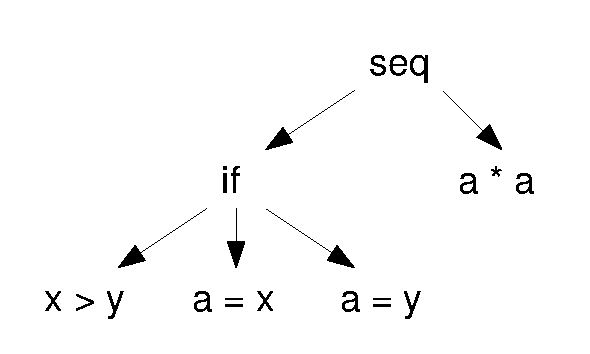
\includegraphics[scale=0.6]{instree.pdf}
  \caption{木構造をした命令}\label{fig:impl-instree}
 \end{center}
\end{minipage}
\begin{minipage}{0.5\hsize}
 \begin{center}
  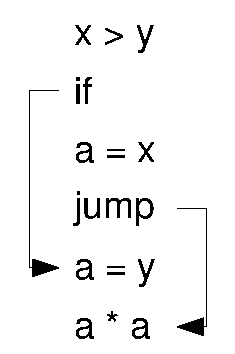
\includegraphics[scale=0.6]{insliner.pdf}
  \caption{直線化した命令}\label{fig:impl-insliner}
 \end{center}
\end{minipage}
\end{figure}


\section{生成するデータ構造}\label{sc:impl-data-structure}%正直位置が微妙
 実行時にメモリ上へ生成するデータ構造:タプルや配列,クロージャについて
 説明する.

\subsection{データ型の表現}
プログラム中のデータは大きく次の2通りに分かれる.
\begin{itemize}
 \item \typename{int}や\typename{float}などの基底型
 \item タプルや配列などの複合型
\end{itemize}

基底型は目的とする計算機に対して自然な表現を採用する.たとえば
\typename{int}型はマシンワード\footnote{ある計算機にとってもっとも扱いや
すいビット幅のこと.IA-32アーキテクチャならば32ビット幅となる.}と等しい
ビット幅を持ち``タグ''などが付加されることはない.また全て値型であり,直
接スタックやレジスタに置かれる.\typename{float}型には倍精度浮動小数点数
を採用した.これもスタックやレジスタに直接確保される.

タプルと配列はヘッダとして,長さやデータがポインタであるかを示すLayout
Bitmap\cite{Nguyen:2006:CMP:1140335.1140364}を持つ.これは,将来的にガベー
ジコレクタを実装する為に使用し,また比較演算の実装に用いる(詳しくは
\refSc{sc:impl-runtime}を参照のこと).

クロージャは先頭に関数のアドレス,続きに自由変数の値を持つタプルとして表
現される.ヴァリアントは型構築子を示す整数と後続にデータ本体を持つ``ドッ
トリスト''のように表現される.


\section{命令選択部}\label{sc:impl-inst}
 一旦,データを割付けるレジスタを決定しないままにIA-32アーキテクチャに存
 在する命令に仮想機械語を変換する.仮想機械語では独立したデスティネーショ
 ンオペランドを持つが,IA-32アーキテクチャでは2オペランドの片側が兼用に
 なっている命令が殆どである.元の値を保存する必要があるため,データの複
 製を行い,そのコピーに対して演算を行うようにした.

 一部の命令は使用できるレジスタが固定であるので,それはこの段階で割り当
 てることとした.それには呼び出し規約を満足させるために,戻り値を適切な
 レジスタに移動することも含む.

 また一部の命令に対しては,演算強度の低減に当たるような命令選択も行なっ
 ている.


\section{レジスタ割り当て}\label{sc:impl-regalloc}
 まず,末尾から走査することで,ある命令の実行時点で生存している一時変数の
 一覧を作成する.その後,上から飽食的に一時変数へレジスタを割り当ててい
 く.制御フローの合流地点においては,生存している変数を全てスタックフレー
 ム上に割り当てることで相互間でのレジスタの位置合せを軽減する.

 できる限り寿命となった変数の割り当てられたレジスタから優先的に使用する
 ことでレジスタ間転送を削減させる.

 レジスタ割り当てを実行し,スタックにスピルするデータを決定したことでス
 タックへ確保する駆動フレームのサイズと値の型がわかる.これを用い
 て,\lstinline|Entry|というスタブの位置にスタックフレームを確保する命令
 を挿入する.

 2011年2月3日時点,まだRegAllocモジュールは実装されていない.このため,
 現在出力できるアセンブリ言語ではレジスタ名のかわりに一時変数名が出力さ
 れる.


\section{実行時ランタイム}\label{sc:impl-runtime}
 実行時に必要となるライブラリには次のものがある.
\begin{itemize}
 \item メモリ管理機構
 \item 複合型に対する比較器
 \item エントリーポイントとなるmain関数
\end{itemize}
 
 2011年2月3日時点,実行時ランタイムとなるCプログラムは実装されていない.

\subsection{メモリ管理機構}
メモリ管理部は,プログラムの実行開始してすぐにタプルや配列を割付けるヒー
プを確保する.管理の都合から次の3種に分けて確保する.
\begin{itemize}
 \item 標準的なサイズのデータ\footnote{\typename{int}型以下のサイズを持
       つ値のことを指す.これにはポインタも含む.}を持つリスト領域
 \item 大きなサイズのデータ\footnote{\typename{float}型のことを指す.}を
       持つリスト領域
 \item その他,タプルと配列の領域
\end{itemize}

これに加え,標準的なサイズのデータのリスト領域に対しては,データ部がポイ
ンタであるかを示すbitmapを領域全体に対して用意する.

また,それぞれの領域に必要なだけメモリを確保するアロケータが必要である.
アロケータは確保したいデータの種類ごとに用意される.それぞれは必要なメモ
リ領域を引数に取るが,タプルや配列を確保するアロケータは,ヘッダ部分のメ
モリ領域を追加しただけのメモリを割り当てる.そして,ヘッダ領域は返される
ポインタより前の部分置く.こうしてポインタが直接データ本体を指すようにす
ることで,データアクセスを単純かつ高速になるようにする.

\subsection{複合型に対する比較器}
一般にポインタの内部を比較するとき,関数の特殊化の都合から内部のデータ構
造をコンパイル時に知ることができない.そのため,ヘッダ部分を見ながら比較
を行う関数を作成することとした.リストであるかどうかは,ポインタが指す領
域を比較することで判定ができる.タプルか配列であるかはヘッダの構造からわ
かる.ポインタかどうかも同様である.これらを使うことで同一であるかの判定
をすることができる.

\subsection{エントリーポイントとなる関数}
メモリ管理機構を起動し,トップレベル変数の束縛を順に行う関数を呼び出すエ
ントリーポイントとなる関数はC言語で作成する.


\chapter{サンプルプログラムと実行結果}\label{ch:sample-program}
ユークリッドの互除法に似た,2つの整数の最大公約数を求める関数を例に
nibkameコンパイラの動作を説明する.このサンプルプログラムを
\refFig{fig:impl-sample}に表す.構文解析を実施しS式表現へ変換すると
\refFig{fig:impl-s-sample}となる.
\begin{figure}[htb]
\begin{minipage}{0.5\hsize}
 \begin{center} 
 \begin{lstlisting}
 let rec gcd = fun m n ->
 if m = 0
 then n
 else if m <= n then
   gcd m (n - m)
 else
   gcd n (m - n)   
 \end{lstlisting}
 \caption{最大公約数を求める関数}\label{fig:impl-sample}
 \end{center}
\end{minipage}
\begin{minipage}{0.5\hsize} 
 \begin{center} 
 \begin{lstlisting}[language=lisp]
 (letrec gcd
   (fun (m n)
     (if (= m 0)
       n
       (if (<= m n)
         (gcd m (- n m))
         (gcd n (- m n))))))  
 \end{lstlisting}
 \caption{最大公約数を求める関数(S式表現)}\label{fig:impl-s-sample}
 \end{center}
\end{minipage}
\end{figure}

これをクロージャ変換すると\refFig{fig:impl-sample-closure}となる.さらに
仮想機械語へ変換すると\refFig{fig:impl-va-sample}になる.この段階で実行
開始地点となるnibkame\_entry関数が生成されている.これを線形化すると
\refFig{fig:impl-sample-liner}になる.この段階でifの中から式は消えて,所々
にラベルと無条件ジャンプが挿入されている.
これにIA-32アーキテクチャの持つ命令を割り当てて出力すると
\refFig{fig:imple-sample-asm}となる.この段階ではまだレジスタ割り当てが行
われていないので,レジスタ名でなく一時変数名が出力されている.現状で実装
されているのは以上となる.

\begin{figure}[htb]
\begin{center} 
\begin{lstlisting}
  Closure.FunDecl
   {Closure.fun_name =
     (Id.L ``gcd'', Type.Fun ([Type.Int; Type.Int], Type.Int));
    Closure.args = [(``m'', Type.Int); (``n'', Type.Int)];
    Closure.formal_fv = [];
    Closure.body =
     Closure.Let ((``t'', Type.Int), Closure.Int 0,
      Closure.If (Closure.Eq, ``m'', ``t'', Closure.Var ``n'',
       Closure.If (Closure.LsEq, ``m'', ``n'',
        Closure.Let ((``r'', Type.Int), Closure.Sub (``n'', ``m''),
         Closure.ApplyDir
          ((Id.L ``gcd'', Type.Fun ([Type.Int; Type.Int], Type.Int)),
          [''m''; ``r''])),
        Closure.Let ((``r2'', Type.Int), Closure.Sub (``m'', ``n''),
         Closure.ApplyDir
          ((Id.L ``gcd'', Type.Fun ([Type.Int; Type.Int], Type.Int)),
          [''n''; ``r2''])))))}
\end{lstlisting}
\caption{クロージャ変換された関数}\label{fig:impl-sample-closure}
\end{center}
\end{figure}

\begin{figure}[htb]
\begin{center}
\begin{lstlisting}
  [{VirtualAsm.name = Id.L ``nibkame_entry''; VirtualAsm.args = [];
    VirtualAsm.body = VirtualAsm.Ans (VirtualAsm.Set (VirtualAsm.Int_l 0));
    VirtualAsm.ret = VirtualAsm.Int};
   {VirtualAsm.name = Id.L ``gcd'';
    VirtualAsm.args = [(``m'', VirtualAsm.Int); (``n'',
   VirtualAsm.Int)];
    VirtualAsm.body =
     VirtualAsm.Let ((``t'', VirtualAsm.Int),
      VirtualAsm.Set (VirtualAsm.Int_l 0),
      VirtualAsm.Ans
       (VirtualAsm.If
         (VirtualAsm.Comp (VirtualAsm.Eq, VirtualAsm.Int, ``m'', VirtualAsm.V ``t''),
         VirtualAsm.Ans (VirtualAsm.Mov (VirtualAsm.V ``n'')),
         VirtualAsm.Ans
          (VirtualAsm.If
            (VirtualAsm.Comp (VirtualAsm.LsEq, VirtualAsm.Int, ``m'',
              VirtualAsm.V ``n''),
            VirtualAsm.Let ((``r'', VirtualAsm.Int),
             VirtualAsm.Sub (``n'', VirtualAsm.V ``m''),
             VirtualAsm.Ans
              (VirtualAsm.ApplyDir
                ((Id.L ``gcd'',
                  VirtualAsm.Fun ([VirtualAsm.Int; VirtualAsm.Int],
                   VirtualAsm.Int)),
                [''m''; ``r'']))),
            VirtualAsm.Let ((``r2'', VirtualAsm.Int),
             VirtualAsm.Sub (``m'', VirtualAsm.V ``n''),
             VirtualAsm.Ans
              (VirtualAsm.ApplyDir
                ((Id.L ``gcd'',
                  VirtualAsm.Fun ([VirtualAsm.Int; VirtualAsm.Int],
                   VirtualAsm.Int)),
                [''n''; ``r2'']))))))));
    VirtualAsm.ret = VirtualAsm.Int}]
  \end{lstlisting}
\caption{仮想機械語のgcd関数}\label{fig:impl-va-sample}
 \end{center}
\end{figure}

\begin{figure}[htb]
\begin{center}
\begin{lstlisting}
  [{Basicblock.name = Id.L ``nibkame_entry''; Basicblock.args = [];
    Basicblock.body =
     [Basicblock.Label (Id.L ``nibkame_entry''); Basicblock.Entry;
      Basicblock.Set (VirtualAsm.Int_l 0); Basicblock.Ret];
    Basicblock.ret = VirtualAsm.Int; Basicblock.block_labels = []};
   {Basicblock.name = Id.L ``gcd'';
    Basicblock.args = [(``m'', VirtualAsm.Int); (``n'', VirtualAsm.Int)];
    Basicblock.body =
     [Basicblock.Label (Id.L ``gcd''); Basicblock.Entry;
      Basicblock.Let ((``t'', VirtualAsm.Int),
       Basicblock.Set (VirtualAsm.Int_l 0));
      Basicblock.If
       (Basicblock.Comp (VirtualAsm.Eq, VirtualAsm.Int, ``m'',
         VirtualAsm.V ``t''),
       Id.L ``block1'');
      Basicblock.If
       (Basicblock.Comp (VirtualAsm.LsEq, VirtualAsm.Int, ``m'',
         VirtualAsm.V ``n''),
       Id.L ``block2'');
      Basicblock.Let ((``r2'', VirtualAsm.Int),
       Basicblock.Sub (``m'', VirtualAsm.V ``n''));
      Basicblock.ApplyDir
       ((Id.L ``gcd'',
         VirtualAsm.Fun ([VirtualAsm.Int; VirtualAsm.Int], VirtualAsm.Int)),
       [''n''; ``r2'']);
      Basicblock.Ret; Basicblock.Label (Id.L ``block2'');
      Basicblock.Let ((``r'', VirtualAsm.Int),
       Basicblock.Sub (``n'', VirtualAsm.V ``m''));
      Basicblock.ApplyDir
       ((Id.L ``gcd'',
         VirtualAsm.Fun ([VirtualAsm.Int; VirtualAsm.Int], VirtualAsm.Int)),
       [''m''; ``r'']);
      Basicblock.Ret; Basicblock.Label (Id.L ``block1'');
      Basicblock.Mov (VirtualAsm.V ``n''); Basicblock.Ret];
    Basicblock.ret = VirtualAsm.Int;
    Basicblock.block_labels = [Id.L ``block2''; Id.L ``block1'']}]
\end{lstlisting}
\end{center}
\caption{線形化された仮想機械語}\label{fig:impl-sample-liner}
\end{figure}

\begin{figure}[htb]
\begin{center}
\begin{lstlisting}
.global gcd

gcd:
# function entry.
movl $0, TempR.t
cmp TempR.t, TempR.m
je block1
cmp TempR.n, TempR.m
jle block2
movl TempR.m, TempR.r2
subl TempR.n, TempR.r2
pushl TempR.r2
pushl TempR.n
call gcd
addl $8, %esp
movl %eax, TempR.tmp5
leave
ret
block2:
movl TempR.n, TempR.r
subl TempR.m, TempR.r
pushl TempR.r
pushl TempR.m
call gcd
addl $8, %esp
movl %eax, TempR.tmp6
leave
ret
block1:
movl TempR.n, TempR.tmp7
leave
ret
\end{lstlisting}
\caption{生成される機械語}\label{fig:imple-sample-asm}
\end{center}
\end{figure}


%\chapter*{謝辞}
\addcontentsline{toc}{chapter}{謝辞}
\section*{謝辞}
樋口先生にはプロジェクト計画についてご意見をいただきました.大墳先生には発表
資料の作成や発表についてご指導いただきました.牛田先生には予稿などの書法につ
いて助言をいただきました.深謝の意を表します.

\bibliographystyle{jplain}
\bibliography{reference}

\backmatter
\appendix

\end{document}
